\subsection{Define the task}
Before getting into more details in the \ref{sec:methodology} section, let's first define the task we will try to learn in this project. Semantic segmentation is a computer vision task where the model learns the general representation of an image by attributing a label to each and every pixels. Intuitively, to make pixel-wise predictions, you first need to have attributed a class to each pixel in the image (see figure \ref{fig:mask}), this is called a \textbf{mask}.

\begin{figure}[H]
	\centering
	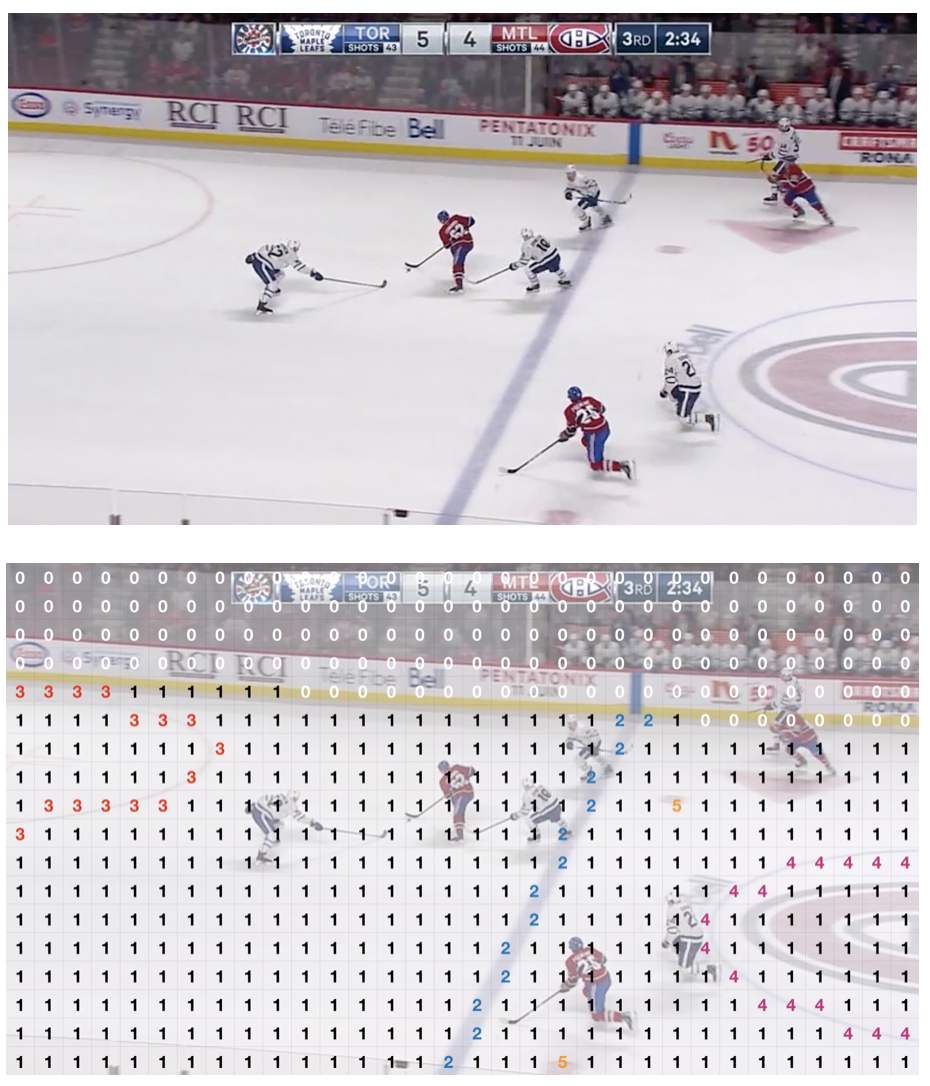
\includegraphics[width=5.5cm, height=5cm]{figures/mask-example.png}
	\caption{Example of mask where each pixel of an image is associated with one class.}
	\label{fig:mask}
\end{figure}

\subsection{Complete workflow}
Once we have a class to every pixel, we now have the output we would like our model to predict. Similarly to other multiclass learning problems, we will have to \textit{one-hot encode} the output of the model so that the output for every pixel will be a vector with the same length as the number of classes. If we look at it matrix-wise instead of pixel-wise, we can say that we will have \textit{one-hot encoded matrix} as the output of the model. Each of those matrix. have the same width and height as the input image, will be related to a specific class and the values predicted by the model will correspond to probabilities to be part of that class.

\begin{figure}[H]
	\centering
	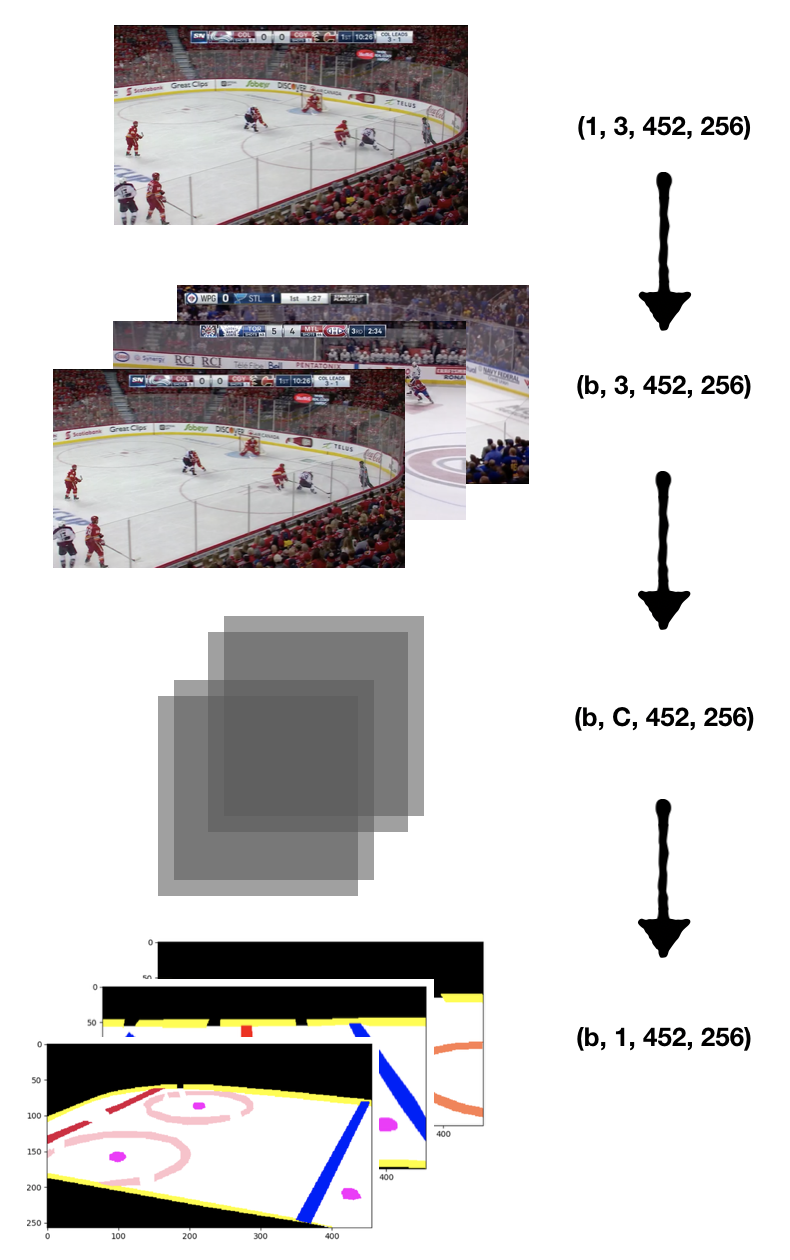
\includegraphics[width=5.5cm, height=10cm]{figures/workflow-dimensions.png}
	\caption{Summary of the workflow behind the semantic segmentation learning task.}
	\label{fig:workflow}
\end{figure}

The figure \ref{fig:workflow} summarizes this workflow where we start from multiple images and ends up with multiple predictions. As such, we start with one RGB image, then we have b images inside one minibatch. At the end of the model, each of those images are \textit{one-hot} encoded to C dimensions, corresponding to the number of classes to predict. Finally, we apply a \texttt{softmax} or any other function that select a predicted class, so that we no longer have C dimensions, but only 1.

